\documentclass[notheorems, 9pt]{beamer}

% Packages with options
\usepackage[english]{babel}
\usepackage[mathscr]{euscript}
\usepackage[utf8]{inputenc}

% Primary Packages
\usepackage{amsbsy, amsmath, amssymb, amsthm, bm, cancel, commath, chngcntr, dsfont, econometrics, gensymb, graphicx, IEEEtrantools, longtable, marginnote, mathrsfs, mathtools, mdframed, natbib, parskip, pgf, setspace, subfigure, tabularx, textcomp, tikz}

% Rest of the setup is in the "setup_beamer" package
\usepackage{setup_beamer}

% Title, Author, Institute
\title{Econ 103: Introduction to Simple Linear Regression}
\author{Manu Navjeevan}
\institute{UCLA}

%%%%%%%%%%%%%%%%%%%%%%%%%%%%%%%%%%%%%%%%%%%%%

\begin{document}
\frame{\titlepage}
\begin{frame}{Content Outline} 
	\label{frame:content-outline}
\end{frame}
\section{The Basic Model}
\begin{frame}{Linear Regression as Line of Best Fit} 
	\label{frame:estimand}
	\onslide<+->
	Suppose we have two variables, \(Y\) and \(X\). We are interested in using data to learning about the relationship between \(Y\) and \(X\).
	
	\onslide<+->
	\red{Examples:}
	\begin{itemize}
		\item How are education and wages related?
		\item<+-> How are unemployment and inflation related?
		\item<+-> What is the relationship between receiving a treatment and a health outcome?
	\end{itemize}
	
\end{frame}
\begin{frame}{Linear Regression as Line of Best Fit} 
	\label{frame:estimand-1}
	One way to model the relationship between \(Y\) and \(X\) would be to try to find the \red{line of best fit} between the two variables. 

	By the \red{line of best fit} we mean finding the line, characterized by a slope and an intercept, that minimizes the distance between \(Y\) and \(\tilde \beta_0 + \tilde\beta_1 \cdot X\).

	\onslide<2->
	Formally, we are interested in the parameters \(\ucla{\beta_0}\) and \(\ucla{\beta_1}\) that solve
	\begin{align*}
		\ucla{\beta_0}, \ucla{\beta_1} &= \arg\min_{\tilde\beta_0,\tilde\beta_1} \E\left[\left(Y - (\tilde\beta_0 + \tilde\beta_1\cdot X)\right)^2\right] \\
									   &= \arg\min_{\tilde\beta_0,\tilde\beta_1} \E\left[\left(Y - \tilde\beta_0 -\tilde\beta_1 \cdot X\right)^2\right]
	\end{align*} 

\end{frame}
\begin{frame}{Linear Regression as Line of Best Fit} 
	\label{frame:estimand-x}
	\semitransp{One way to model the relationship between \(Y\) and \(X\) would be to try to find the line of best fit between the two variables. 

	By the line of best fit we mean finding the line, characterized by a slope and an intercept, that minimizes the distance between \(Y\) and \(\tilde \beta_0 + \tilde\beta_1 \cdot X\).

	Formally, we are interested in the parameters \(\beta_0\) and \(\beta_1\) that solve
	\begin{align*}
		\beta_0, \beta_1 &= \arg\min_{\tilde\beta_0,\tilde\beta_1} \E\left[\left(Y - (\tilde\beta_0 + \tilde\beta_1\cdot X)\right)^2\right] \\
									   &= \arg\min_{\tilde\beta_0,\tilde\beta_1} \E\left[\left(Y - \tilde\beta_0 -\tilde\beta_1 \cdot X\right)^2\right]
	\end{align*}}
	\noindent\darkucla{\rule{2cm}{0.5pt}}
	\begin{itemize}
		\item<1|only@1> By \(\arg\min\) we just mean we are interested in the \green{\bf arguments} \(\ucla{\beta_0}\) and  \(\ucla{\beta_1}\) that minimize 
		\[
				\E[(Y-\tilde\beta_0-\tilde\beta_1\cdot X)^2]
		\] 
		rather than the value \(\E[(Y-\beta_0-\beta_1\cdot X)^2]\) itself.
		\item<2|only@2> Another way of saying this is that 
		\[
			\E[(Y- \ucla{\beta_0} - \ucla{\beta_1}\cdot X)^2] < \E[(Y - \ucla{\tilde\beta_0} - \ucla{\tilde\beta_1}\cdot X)^2]
		\]
		for any \((\ucla{\tilde\beta_0},\ucla{\tilde\beta_1})\neq (\ucla{\beta_0},\ucla{\beta_1})\).
	\end{itemize}
\end{frame}
\begin{frame}{Linear Regression as Line of Best Fit} 
	\label{frame:estimand-2}
	We are interested in the parameters \(\ucla{\beta_0}\) and \(\ucla{\beta_1}\) that solve
	\begin{align*}
		\ucla{\beta_0}, \ucla{\beta_1} &= \arg\min_{\tilde\beta_0,\tilde\beta_1} \E\left[\left(Y - \tilde\beta_0 -\tilde\beta_1 \cdot X\right)^2\right]
	\end{align*}
	\red{Why do we care about these parameters?}
	\only<1>{
	\begin{itemize}
		\item<1> Knowing the line of best fit will help us predict \(Y\) using \(X\)
		\begin{itemize}
			\item<1> Will provide the \green{best linear prediction} of \(Y\) using \(X\).
			\item<1> Even though a linear model may seem to simple, ends up being tremendously useful in practice.
		\end{itemize}
	\end{itemize}}
	\only<2->{
	\begin{itemize}
	\item<2-> We can also interpret the parameters \(\beta_0\) and  \(\beta_1\) to learn (\green{to a first order degree}) about the relationship between  \(Y\) and \(X\) 
		\begin{itemize}
			\item<3-> Is there a positive or negative relationship between \(Y\) and \(X\)? \(\iff\) Is \(\beta_1\) positive or negative?
			\item<4-> How much can we expect \(Y\) to change if we see an increase in \(X\) of one unit?  \(\iff\) What is  \(\beta_1\)?
			\item<5-> What is the average value of \(Y\) when \(X\) is zero? \(\iff\) What is \(\beta_0\)?
			\item<6-> \green{To a first order degree} because \(\ucla{\beta_0}\) and \(\ucla{\beta_1}\) describe the line of best fit rather than the ``true'' relationship.
			\begin{itemize}
				\item No need to worry about this difference for now though.
			\end{itemize}
		\end{itemize}
	\end{itemize}}
\end{frame}
\begin{frame}{Linear Regression: The Parameters} 
	\label{frame:estimand-3}
	\onslide<+->
	We are interested in the parameters \(\ucla{\beta_0}\) and \(\ucla{\beta_1}\) that solve
	\begin{align*}
		\ucla{\beta_0}, \ucla{\beta_1} &= \arg\min_{\tilde\beta_0,\tilde\beta_1} \E\left[\left(Y - \tilde\beta_0 -\tilde\beta_1 \cdot X\right)^2\right]
	\end{align*}	
	\onslide<+->
	Let's solve for \(\ucla{\beta_0}\) and  \(\ucla{\beta_1}\) by taking first order conditions:
	\begin{align*}
		\frac{\partial }{\partial \tilde\beta_0}:  \E\left[Y-\ucla{\beta_0}- \ucla{\beta_1}\cdot X\right] &= 0 \\ 
		\frac{\partial }{\partial \tilde\beta_1}: \E\left[(Y-\ucla{\beta_0}-\ucla{\beta_1}\cdot X)\cdot X\right] &= 0
	\end{align*}
	\onslide<+->
	We will return to these first order conditions shortly. For now, after rearranging we get that
	\begin{align*}
		\ucla{\beta_1} &= \frac{\E[YX]-\E[Y]\E[X]}{\E[X^2]-\E[X]\E[X]} = \frac{\Cov(Y,X)}{\Var(X)}   \\
		\ucla{\beta_0} &= \E[Y] - \ucla{\beta_1}\E[X]
	\end{align*}
	\onslide<+->
	\green{Exercise: Show this rearrangement.}
\end{frame}
\begin{frame}{Linear Regression: The Error Term} 
	\label{frame:eps-1}
	Let's define the random variable
	\begin{align*}
		\eps &= Y - (\ucla{\beta_0} + \ucla{\beta_1}\cdot X) \\
			 &= Y - \ucla{\beta_0} - \ucla{\beta_1}\cdot X
	\end{align*} 
	\onslide<+->
	We can then write
	\[
		Y = \ucla{\beta_0} + \ucla{\beta_1}\cdot X + \eps
	.\] 
	which is the linear regression equation you may have seen before. The random variable \(\eps\) will be important later on as we try to do inference.
\end{frame}
\begin{frame}{Linear Regression: The Error Term} 
	\label{frame:eps-2}
	Let's define the random variable
	\begin{align*}
		\eps &= Y - (\ucla{\beta_0} + \ucla{\beta_1}\cdot X) \\
			 &= Y - \ucla{\beta_0} - \ucla{\beta_1}\cdot X
	\end{align*} 
	We call \(\eps\) the  \red{linear regression error} variable. 

	\onslide<2->
	Recall that from the first order conditions for \(\ucla{\beta_0}\) and  \(\ucla{\beta_1}\) we have that
	\begin{align*}
		\E\big[\underbrace{Y-\ucla{\beta_0}- \ucla{\beta_1}\cdot X}_{=\eps}\big] &= 0 \\ 
		\E\big[\underbrace{(Y-\ucla{\beta_0}-\ucla{\beta_1}\cdot X)}_{=\eps}\cdot X\big] &= 0
	\end{align*}
	\onslide<2->
	These give us the properties that
	\[
		\E[\eps]= 0\andbox \E[\eps X] = 0
	.\] 
\end{frame}
%TODO: Add a slide explaining how sometimes people give interpretations to error terms and it's importance to causal inference.
%TODO: Add a slide and discuss the variance of the error term as well as the conditional variance.

\begin{frame}{Linear Regression: Model Summary} 
	\label{frame:model-summary}
	In total our \red{line of best fit} parameters
	\begin{align*}
		\ucla{\beta_0}, \ucla{\beta_1} &= \arg\min_{\tilde\beta_0,\tilde\beta_1} \E\left[\left(Y - \tilde\beta_0 -\tilde\beta_1 \cdot X\right)^2\right]
	\end{align*}
	generate a model betwen \(Y\) and \(X\) that can be written as 
	\begin{equation}
		Y = \ucla{\beta_0} + \ucla{\beta_1}\cdot X + \eps
	\end{equation} 
	where 
	\[
		\E[\eps]= 0 \andbox \E[\eps X]=0
	.\]
	\onslide<2->
	\begin{itemize}
		\item It is often convenient to work directly with this representation or make assumptions about \(\eps\).
		\item You may have seen this representation before, the prior slides go over where this model comes from
	\end{itemize}
\end{frame}

\begin{frame}{Linear Regression: Model Summary} 
	\label{frame:model-summary-2}
	Our \red{line of best fit} parameters
	\begin{align*}
		\ucla{\beta_0}, \ucla{\beta_1} &= \arg\min_{\tilde\beta_0,\tilde\beta_1} \E\left[\left(Y - \tilde\beta_0 -\tilde\beta_1 \cdot X\right)^2\right]
	\end{align*}
	are useful for 
	\begin{itemize}
		\item<1-> Making predictions about \(Y\) using  \(X\).
		\begin{itemize}
			\item Predict \(Y\) when  \(X=x\) with  \(\beta_0  + \beta_1\cdot x\)
		\end{itemize}
	 \item<2-> Learning about the relationship between \(Y\) and  \(X\).
	\begin{itemize}
		\item Interpret the signs and magnitudes of \(\beta_0\) and  \(\beta_1\)
	\end{itemize}
	\end{itemize}
\end{frame}
\begin{frame}{Linear Regression: Questions}
	\centering
	\red{\Large Questions?}
\end{frame} 

\section{Estimation}%
\label{sec:estimation}

\begin{frame}{Linear Regression: Estimation Introduction} 
	\label{frame:estimation-intro}
	As we went over in the last section we are interested in the line of best fit parameters
	\begin{align*}
		\ucla{\beta_0}, \ucla{\beta_1} &= \arg\min_{\tilde\beta_0,\tilde\beta_1} \E\left[\left(Y - \tilde\beta_0 -\tilde\beta_1 \cdot X\right)^2\right]
	\end{align*}
	\red{Problem:} We do not know know the joint distribution of \((Y,X)\), so we cannot to solve for \(\beta_0\) and  \(\beta_1\) by evaluating the expectation above. 

	\onslide<2->
	\red{Solution:} Use data to estimate the parameters \(\ucla{\beta_0}\) and  \(\ucla{\beta_1}\).
\end{frame}
\begin{frame}{Linear Regression: The Estimator} 
	\label{frame:estimator-intro}
	\red{Solution:} Use data to try and estimate the parameters \(\ucla{\beta_0}\) and  \(\ucla{\beta_1}\).

	How do we do this?
	\onslide<2->

	\ucla{Intuition:}
	\begin{itemize}
		\item<2-> Suppose we have access to \(n\) randomly collected samples  \(\{Y_i,X_i\}_{i=1}^n\)
		\item<3-> We are interested in the line of best fit between \(Y\) and \(X\) in the population
		\begin{align*}
			\ucla{\beta_0}, \ucla{\beta_1} = \arg\min_{\tilde\beta_0,\tilde\beta_1} \E\left[\left(Y - \tilde\beta_0 -\tilde\beta_1 \cdot X\right)^2\right]
		\end{align*}
		\only<4>{\item We estimate the line of best fit between \(Y\) and \(X\) in the population using the line of best fit between \(Y_i\) and \(X_i\) in our sample:
		\begin{align*}
			\ucla{\hat\beta_0},\ucla{\hat\beta_1} = \arg\min_{b_0,b_1} \frac{1}{n} \sum_{i=1}^n \left(Y_i - b_0 - b_1\cdot X_i\right)^2
		\end{align*}
		\begin{itemize}
			\item Same idea as using \(\bar X\) to estimate  \(\E[X]\), etc.
		\end{itemize}}
		\only<5>{\item We estimate the line of best fit between \(Y\) and \(X\) in the population using the line of best fit between \(Y_i\) and \(X_i\) in our sample:
		\begin{align*}
			\ucla{\hat\beta_0},\ucla{\hat\beta_1} = \arg\min_{b_0,b_1} \cancel{\frac{1}{n}} \sum_{i=1}^n \left(Y_i - b_0 - b_1\cdot X_i\right)^2
		\end{align*}
		\begin{itemize}
			\item Same idea as using \(\bar X\) to estimate  \(\E[X]\), etc.
		\end{itemize}}
	\end{itemize}
\end{frame}
\begin{frame}{Linear Regression: The Estimator} 
	\label{frame:estimator-visualization}
	Let's see how this looks like in practice. Suppose we are interested in the relationship between \(X\), a car's weight, and \(Y\) a car's miles per gallon (mpg). 

	We collect some data \(\{Y_i,X_i\}_{i=1}^n\) where each \((Y_i,X_i)\) pair represents the miles per gallon and weight of a particular vehicle in our dataset. We can represent our data using a scatterplot
	\begin{figure}[htpb]
		\centering
		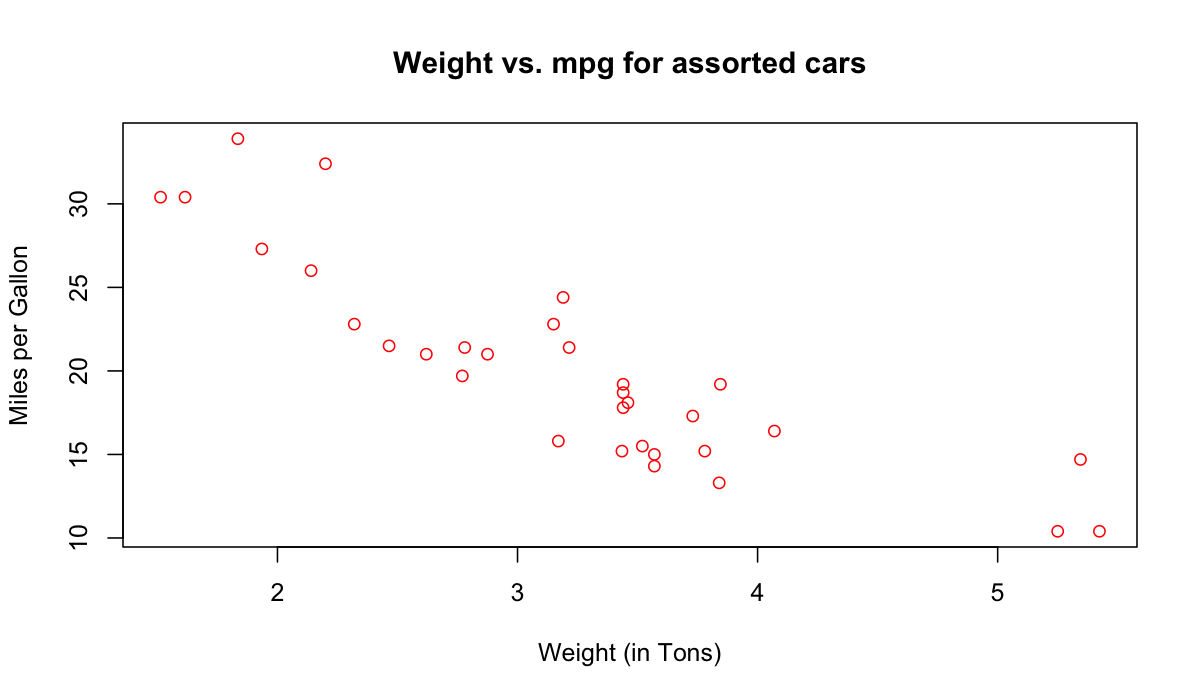
\includegraphics[width=0.8\linewidth]{scatter1.png}		
	\end{figure}
\end{frame}
\begin{frame}{Linear Regression: The Estimator} 
	\label{frame:estimator-visualization-2}
	Now to estimate \(\ucla{\hat\beta_0}, \ucla{\hat\beta_1}\) we simply find the line of best fit between the \(Y_i\) and \(X_i\) 's in our data. 
	\begin{figure}[htpb]
		\centering
		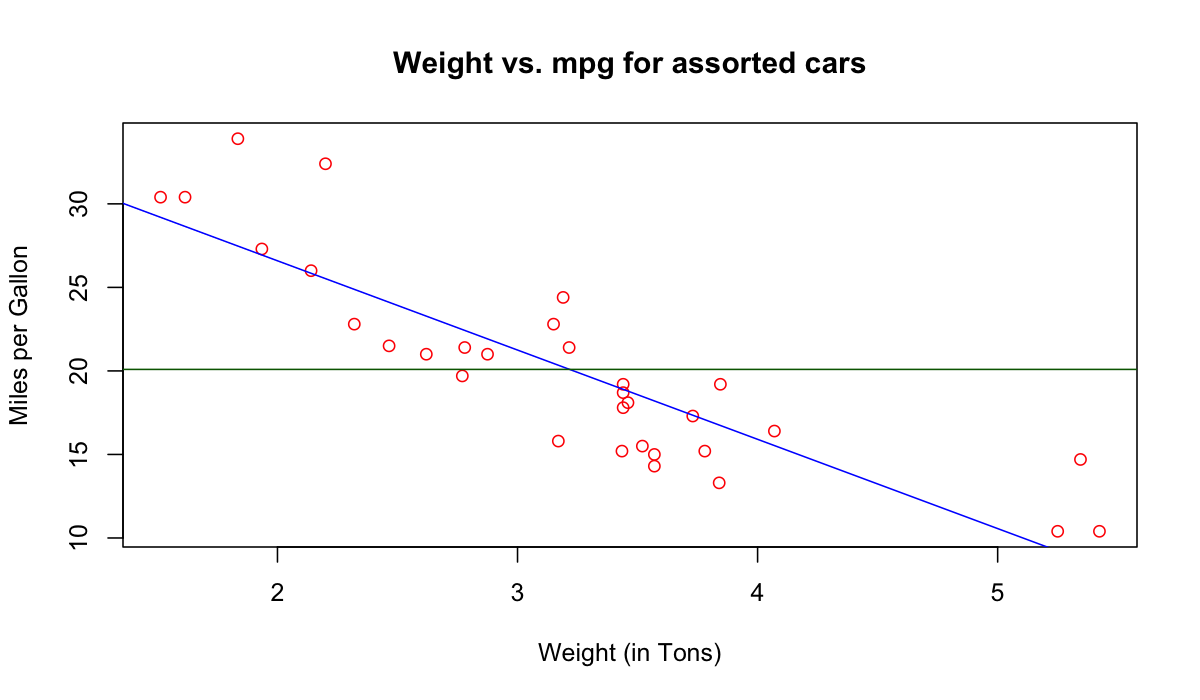
\includegraphics[width=0.8\linewidth]{scatter2.png}
	\end{figure}
	\only<2>{
	The \darkucla{blue} line represents the line of best fit whereas the \green{green} line represents a straight line through \(\bar Y\). We can see that the \darkucla{blue} line is much closer to the data than the \green{green} line.}
\end{frame}

\begin{frame}{Linear Regression: The Estimator} 
	\label{frame:estimator-2}

	In this case we have that \(\ucla{\hat\beta_0} = 37.2851\) and \(\ucla{\hat\beta_1} = -5.3445.\)

	\red{How do we interpret these estimates?}
	\begin{itemize}
		\item<2-> \(\ucla{\hat\beta_0} = 37.2851\): We estimate that the average value of  \(Y\) when  \(X=0\) is  \(37.2851\)
		\begin{itemize}
			\item In context: we estimate that the average mpg for a car that weights \(0\) tons is  \(37.2851\) miles per gallon
		\end{itemize}
		\item<3-> \(\ucla{\hat\beta_1}= -5.3445\): We estimate that, on average, a one unit increase in  \(X\) is associated with a  \(5.3445\) unit \ucla{decrease} in  \(Y\).
		\begin{itemize}
			\item In context: we estimate that, on average, a one ton increase in car weight is associated with a 5.3445 unit decrease in miles per gallon.
		\end{itemize}
	\end{itemize}
\end{frame}
\begin{frame}{Linear Regression: The Estimator} 
	\label{frame:estimator-3}
	In this case we have that \(\ucla{\hat\beta_0} = 37.2851\) and \(\ucla{\hat\beta_1} = -5.3445.\)

	\red{How can we use these estimates for prediction?}
	\begin{itemize}
		\item Suppose we have a car that weighs \(3.5\) tons. Based on our estimates, what would we predict its miles per gallon to be?
		\begin{itemize}
			\item<2-> Our estimated regression line is 
			\[
				\text{Predicted MPG} = 37.2851 - 5.3445\cdot\text{Weight in Tons}
			.\] 
			\item<3-> Using this line and plugging in we get that 
			\[
				\text{Predicted MPG} = 37.2851 - 5.3445\cdot 3.5 = 18.5793
			.\] 
			\item<4-> We denote this predicted MPG as \(\hat{\text{MPG}}\) and in general will denote our predictions as \(\hat Y\) so that our estimated regression line can be written
			\[
				\hat Y = \ucla{\hat\beta_0} + \ucla{\hat\beta_1}\cdot X
			.\] 
		\end{itemize}
	\end{itemize}
\end{frame}

\begin{frame}{Linear Regression: The Estimator} 
	\label{frame:estimator-4}
	Notice a couple things in the above interpretations
	\begin{itemize}
		\item The intercept is often uninterpretable (\green{What car would weigh 0 tons?}). For this reason we often focus our analysis on the slope coefficient. 
		\item The interpretation is deliberately not \green{causal}. We use ``associated with a decrease\dots'' as opposed to ``leads to a decrease\dots''
		%TODO: Add an explanation here for why we cannot interpret these causally
	\end{itemize} 
\end{frame}

\begin{frame}{Linear Regression: Formulas} 
	\label{frame:estimator-formula}
	Now that we've gotten some intuition for what linear regression is doing and how to use our sample to estimate the parameters of interest, let's derive explicit formulas for \(\ucla{\hat\beta_0}\) and \(\ucla{\hat\beta_1}\).

	\onslide<2->
	Recall that 
	\[
	    \ucla{\hat\beta_0},\ucla{\hat\beta_1} = \arg\min_{b_0,b_1} \frac{1}{n}\sum_{i=1}^n \left(Y_i - b_0 - b_1\cdot X_i\right)^2 
	.\] 
	\onslide<3->
	Taking first order conditions gives us that
	\begin{align*}
		\frac{\partial }{\partial b_0}: \frac{1}{n}\sum_{i=1}^n (Y_i - \ucla{\hat\beta_0} - \ucla{\hat\beta_1}\cdot X_i) &= 0 \\
		\frac{\partial }{\partial b_1}: \frac{1}{n}\sum_{i=1}^n (Y_i - \ucla{\hat\beta_0} - \ucla{\hat\beta_1}\cdot X_i)\cdot X_i &=0
	\end{align*}	
\end{frame}
\begin{frame}{Linear Regression: Formulas} 
	\label{frame:estimator-formula-1}
	Rearranging the first equality gives us
	\begin{align*}
		\frac{1}{n}\sum_{i=1}^n  Y_i - \frac{1}{n}\sum_{i=1}^n \ucla{\hat\beta_0} - \frac{1}{n}\sum_{i=1}^n \ucla{\hat\beta_1}\cdot X_i &= 0 \\
		\onslide<2->{
		\bar Y - \ucla{\hat\beta_0} - \ucla{\hat\beta_1}\frac{1}{n}\sum_{i=1}^n X_i &= 0 \\}
		\onslide<3->{
		\bar Y - \ucla{\hat\beta_0} - \ucla{\hat\beta_1}\bar X &= 0 \\
		\ucla{\hat\beta_0} &= \bar Y - \ucla{\hat\beta_1}\bar X }
	\end{align*}
	\onslide<3->
	So that what remains is to solve for \(\ucla{\hat\beta_1}\).
\end{frame}
\begin{frame}{Linear Regression: Formulas} 
	\label{frame:estimator-formula-2}
	Rearranging the second equality gives us
	\begin{align*}
		\frac{1}{n}\sum_{i=1}^n Y_i X_i - \ucla{\hat\beta_0}\frac{1}{n}\sum_{i=1}^n X_i - \ucla{\hat\beta_1}\frac{1}{n}\sum_{i=1}^n X_i^2 &= 0
		\onslide<2->{
			\intertext{Using the prior result that \( \ucla{\hat\beta_0} = \bar Y - \ucla{\hat\beta_1}\bar X\) gives:}
		\frac{1}{n}\sum_{i=1}^n Y_i X_i - (\bar Y - \ucla{\hat\beta_1}\bar X)\bar X - \ucla{\hat\beta_1}\frac{1}{n}\sum_{i=1}^n X_i^2 &= 0 \\
		\left(\frac{1}{n}\sum_{i=1}^n Y_i X_i - \bar Y \bar X\right) + \ucla{\hat\beta_1}\left((\bar X)^2 - \frac{1}{n}\sum_{i=1}^nX_i^2\right) &=0\\
		}
	\end{align*}
	\onslide<3->
	So, finally
	\[
		\ucla{\hat\beta_1} = \frac{\frac{1}{n}\sum_{i=1}^n Y_i X_i - \bar Y \bar X}{\frac{1}{n}\sum_{i=1}^n X_i^2 - (\bar X)^2} 
	.\] 
\end{frame}
\begin{frame}{Linear Regression: Formulas} 
	\label{frame:estimator-formula-3}
	Let's make use of the following equalities to represent \( \ucla{\hat\beta_1}\)
	%TODO: Assign proving these as a homework exercise
	\begin{align*}
		\frac{1}{n}\sum_{i=1}^n (Y_i - \bar Y)(X_i - \bar X) &= \frac{1}{n}\sum_{i=1}^n  Y_iX_i - \bar Y \bar X \\
		\frac{1}{n}\sum_{i=1}^n (X_i - \bar X)^2 &= \frac{1}{n}\sum_{i=1}^n X_i^2 - (\bar X)^2 
	\end{align*}
	\onslide<2->
	\red{Then:}
	\begin{align*}
		\ucla{\hat\beta_1} = \frac{\overbrace{\frac{1}{n}\sum_{i=1}^n (Y_i - \bar Y)(X_i - \bar X)}^{\text{Sample Covariance between \(Y\) and \(X\)}}}{\underbrace{\frac{1}{n}\sum_{i=1}^n (X_i - \bar X)^2 }_{\text{Sample Variance of \(X\)}}} 
	\end{align*}
	\onslide<3-> 
	This ties in nicely as, if we recall from earlier, we found that
	\[
		\ucla{\beta_1} = \frac{\Cov(Y,X)}{\Var(X)} = \frac{\E[(Y-\mu_Y)(X-\mu_X)]}{\E[(X-\mu_X)^2]} 
	.\] 
\end{frame}


\begin{frame}{Linear Regression: Randomness} 
	We have now gone over how use data to obtain estimates \(\ucla{\hat\beta_0}, \ucla{\hat\beta_1}\) of our parameters of interest \(\ucla{\beta_0}, \ucla{\beta_1}\).	
	\only<1>{
	\begin{align*}
		\ucla{\hat\beta_0},\ucla{\hat\beta_1} &= \arg\min_{b_0,b_1} \frac{1}{n}\sum_{i=1}^n \left(Y_i - b_0 - b_1\cdot X_i\right)^2 \\
		\ucla{\beta_0}, \ucla{\beta_1} &= \arg\min_{\tilde\beta_0,\tilde\beta_1} \E\left[\left(Y - \tilde\beta_0 -\tilde\beta_1 \cdot X\right)^2\right]
	\end{align*}
	}
	Notice that, while the parameters of interest \(\ucla{\beta_0}\) and  \(\ucla{\beta_1}\) are fixed quantities, the estimators \(\ucla{\hat\beta_0}\) and  \(\ucla{\hat\beta_1}\) are functions of the data; they depend on the specific sample of data collected.  
	\onslide<2->

	\red{Some Questions to Consider:}
	\begin{enumerate}
		\item<2-> What would happen to our estimates \(\ucla{\hat\beta_0}\) and \(\ucla{\hat\beta_1}\) if we were to collect a different sample of data?
		\item<3-> How can we model the distribution of our estimates \(\ucla{\hat\beta_0}\) and  \(\ucla{\hat\beta_1}\)?
		\item<4-> What happens to this distribution as \(n\to\infty\)?
	\end{enumerate}
\end{frame}
\begin{frame}{Linear Regression: Randomness} 
	\label{frame:randomness-example}
	\red{Question:} What would happen to our estimates \(\ucla{\hat\beta_0}\) and \(\ucla{\hat\beta_1}\) if we were to collect a different sample of data?

	\onslide<2->
	Let's return to the cars data and see how our regression lines look when we consider two different (random) samples.
	\begin{figure}[htpb]
		\centering
		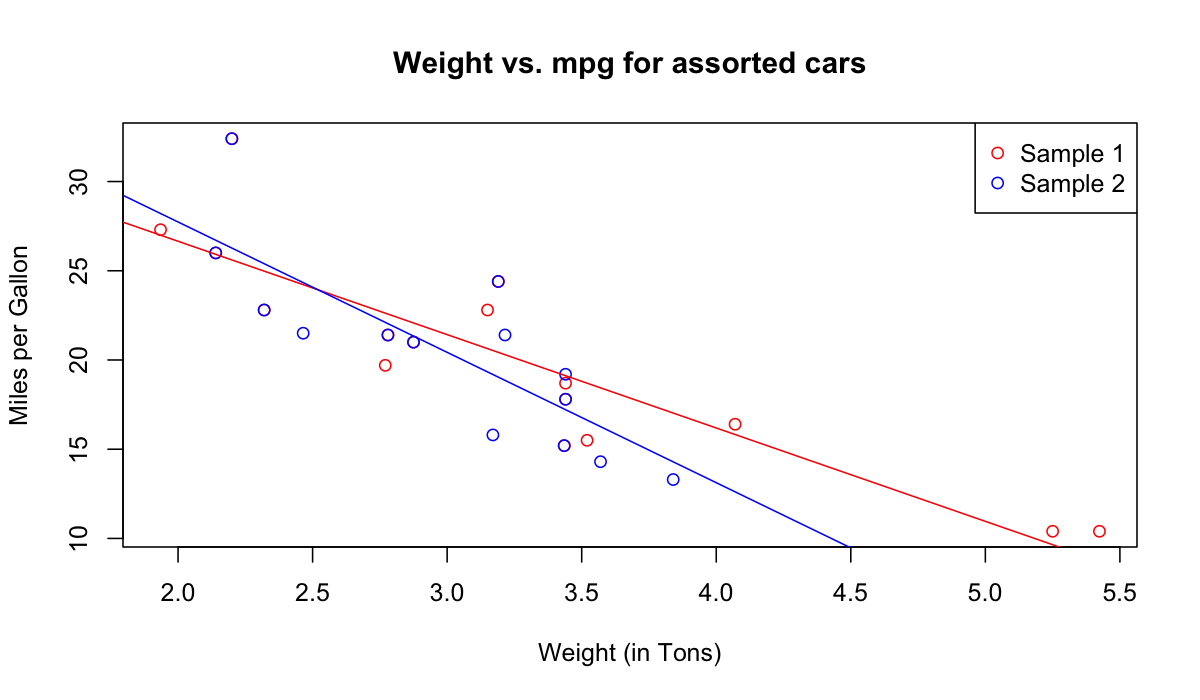
\includegraphics[width=0.75\linewidth]{scatter3.png}	
	\end{figure}
	\onslide<3->
	\begin{itemize}
		\item \red{Sample 1:} \( \ucla{\hat\beta_0} = 37.1285\) and \( \ucla{\hat\beta_1}= -5.2341\).
		\item \darkucla{Sample 2:} \( \ucla{\hat\beta_0} = 42.352\) and \( \ucla{\hat\beta_1} = -7.307\).
	\end{itemize}
\end{frame}
\begin{frame}{Linear Regression: Randomness} 
	\label{frame:randomness-conclusion}
	\ucla{Key Concept:} Because the estimators \(\ucla{\hat\beta_0}\) and \(\ucla{\hat\beta_1}\) are functions of the random sample \(\{Y_i,X_i\}_{i=1}^n\) they are themselves random variables.
	\begin{align*}
		\ucla{\hat\beta_0} &= \bar Y - \ucla{\hat\beta_1}\bar X \\
		\ucla{\hat\beta_1} &= \frac{\frac{1}{n}\sum_{i=1}^n (Y_i - \bar Y)(X_i - \bar X)}{\frac{1}{n}\sum_{i=1}^n (X_i-\bar X)^2} 
	\end{align*}

	\ucla{Problem:} How do we connect \(\ucla{\hat\beta_0}\) and \(\ucla{\hat\beta_1}\) to the population parameters \(\ucla{\beta_0}\) and \(\ucla{\beta_1}\)?
	
	\onslide<2->
	\green{Fundamental Question:} Given estimates \( \ucla{\hat\beta_0}\) and \(\ucla{\hat\beta_1}\) what can we say about the underlying parameters of interest \( \ucla{\beta_0}\) and \(\ucla{\beta_1}\)?
\end{frame}
	
\section{Asymptotic Distribution}%
\label{sec:asymptotic-distribution}

\begin{frame}{Linear Regression: Motivating Idea} 
	\label{frame:motivation}
	Suppose we are interested in the association between years of education and income. We collect a random sample of size \(n = 100\),  \(\{Y_i,X_i\}_{i=1}^{100}\) and run a simple linear regression of \(Y = INC\) against  \(X = EDU\).

	\onslide<2-> 
	That is, we are interested in the parameters \(\ucla{\beta_0}\) and \( \ucla{\beta_1}\) that dictate the line of best fit between income and education in the population
	\[
		\ucla{\beta_0},\ucla{\beta_1} = \arg\min_{\tilde\beta_0,\tilde\beta_1}\E\left[(INC - \tilde\beta_0 - \tilde\beta_1\cdot EDU)^2\right]
	.\]
	or equivalently the parameters from the linear model
	\[
	    INC = \ucla{\beta_0} + \ucla{\beta_1}\cdot EDU + \eps
	.\] 
	where \(\E[\eps \cdot EDU] = 0\).
\end{frame}
\begin{frame}{Linear Regression: Motivating Idea} 
	\label{frame:motivation2}
	Using our data \(\{Y_i,X_i\}_{i=1}^n\) we find that \(\ucla{\hat\beta_1} = 0.5\). 
	\[
		\ucla{\hat\beta_0}\ucla{\hat\beta_1} = \arg\min_{b_0,b_1}\frac{1}{n}\sum_{i=1}^n \left\{Y_i - b_0 - b_1\cdot X_i\right\}^2
	.\] 
	Our friend, Prince Harry Estranged of England, however claims that there is no association between education and income, that is that  \(\ucla{\beta_1} = 0\).	
\end{frame}
\begin{frame}{Linear Regression: Motivating Idea} 
	\label{frame:motivation3}
	\red{Question:} How can we tell if he is right?

	\onslide<2->
	\red{Answer:} One way would be to find the probability that we would obtain \(\ucla{\hat\beta_1}= 0.5\) (or something more extreme) if the true value of \(\ucla{\beta_1}\) was 0.
	\[
		\Pr(|\ucla{\hat\beta_1} | \geq  0.5 | \ucla{\beta_1}= 0)
	.\]  
	If this probability is sufficently low, we can reject Former Prince Harry's claim. Otherwise he may be right. 

	\onslide<3->
	\noindent{\ucla{\rule{2cm}{0.5pt}}}

	To calculate this probability we will need to know something about the (approximate) distribution of \(\ucla{\hat\beta_1}\) and how that is related to the true parameter \( \ucla{\beta_1}\).
\end{frame}

\begin{frame}{Linear Regression: Assumptions} 
	\label{frame:linear-reg-assumptions}
	In order to connect the estimates \(\ucla{\hat\beta_0}\) and \( \ucla{\hat\beta_1}\) to the population parameters, we will need to make some (light) assumptions about the underlying distribution of  \((Y,X)\) from which our sample  \(\{Y_i,X_i\}_{i=1}^n\) is drawn.

	\onslide<2->
	It will be helpful to recall the following definitions here
	\begin{align*}
		\ucla{\beta_0},\ucla{\beta_1} &= \arg\min_{\tilde\beta_0,\tilde\beta_1}\E\left[(Y - \tilde\beta_0 - \tilde\beta_1)^2\right] \\
		\eps &= Y - \ucla{\beta_0} - \ucla{\beta_1}\cdot X
	\end{align*}
	And see that \(\eps\) is itself a random variable. 
\end{frame}

\begin{frame}{Linear Regression: Assumptions} 
	\label{frame:assm-2}
	Make the following assumptions
	\begin{enumerate}
		\item<1-> \darkucla{Random Sampling:} Assume that \(\{Y_i,X_i\}\) are independently and identically distributed; \((Y_i,X_i) \overset{\text{i.i.d}}{\sim} (Y,X)\)
		\begin{itemize}
			\item<1|only@1> Essentially this means that our random sample is ``representative of the population'' 
			\item<1|only@1> Would be violated if say, we only sampled cars made in Los Angeles and we were trying to make inferences about all cars produced in the US
		\end{itemize}
		\item<2-> \darkucla{Homoskedasticity:} Assume that \(\Var(\eps\mid X=x) = \sigma_\eps^2 \) for all possible values of \(x\).
		\begin{itemize}
			\item<2|only@2> This means that \(Y\) is equally spread around the regression line for all values of \(X\).
			\item<2|only@2> This is a fairly strong assumption to make and we will relax it later on, but it is helpful for now to provide insight.
			\item<2|only@2> Conditional variance is similar to the conditional expectation that we went over in our Econ 41 review
			\[
				{\Var(\eps\mid X=x) = \E[\eps^2|X=x] - (\E[\eps|X=x])^2}
			.\] 
			\item<2->An important implication of this is that
			\[
				\Var(\eps(X-\mu_X)) = \Var(\eps)\Var(X) = \sigma_\eps^2\sigma_X^2
			.\] 
			\only<2>{\green{Questions?}}
		\end{itemize}
		\item<3-> \darkucla{Rank Condition:} There must be at least two distinct values of \(X\) that appear in the population.
		\begin{itemize}
			\item<3|only@3> Need at least two distinct points to make a line. 
			\item<3|only@3> If there is only one distinct point then our minimization problem is undefined.
		\end{itemize}
	\end{enumerate}
	\onslide<4->
	And that's it!
\end{frame}
\begin{frame}{Linear Regression: Asymptotic Distribution} 
	\label{frame:asymptotic-dist}
	Given these assumptions (\darkucla{Random Sampling}, \darkucla{Homoskedasticity}, \darkucla{Rank Condition}) let's try and figure out what the approximate distribution is of \(\ucla{\hat\beta_1}\).
	
	Recall that 
	\begin{align*}
		\ucla{\hat\beta_1} = \frac{\frac{1}{n}\sum_{i=1}^n (Y_i-\bar Y)(X_i - \bar X)}{\frac{1}{n}\sum_{i=1}^n (X_i-\bar X)^2} 
	\end{align*}
	\onslide<2->
	By definition of \(\eps = Y - \ucla{\beta_0} - \ucla{\beta_1}\cdot X\):
	\begin{align*}
		Y = \ucla{\beta_0} + \ucla{\beta_1}\cdot X;	
	\end{align*}
	and that by the first order conditions of \(\ucla{\beta_0}\) and \(\ucla{\beta_1}\): 
	\begin{align*}
		\E[\eps] &= 0 \\
		\E[\eps\cdot X] &= 0
	\end{align*}
\end{frame}
\begin{frame}{Linear Regression: Asymptotic Distribution} 
	\label{frame:review-lln-clt}
	We will also make use of the following results from our probability review. If \(Z\) is a random variables and we have i.i.d observations  \(Z_1,Z_2,..,Z_n\):

	The \red{Law of Large Numbers} states that as \(n \to \infty\):
	\[
		 \bar Z \to \E[Z]
	\] 
	or, equivalently, \(\bar Z \approx \E[Z]\) for  \(n\) large.
	\vfill{ }
	The \red{Central Limit Theorem} states that as  \(n\to \infty\), approximately,
	 \[
		 \sqrt{n}\left(\bar Z - \E[Z]\right) \sim N\left(0,\Var(Z)\right)
	\] 
	or, equivalently, \(\bar Z \sim N\left(\E[Z],\Var(Z)/n\right)\).
\end{frame}
\begin{frame}{Linear Regression: Asymptotic Distribution} 
	\label{frame:alt1}
	Starting with:	
	\[
	    \sqrt{n}\ucla{\hat\beta_1} =  \frac{\sqrt{n}\frac{1}{n}\sum_{i=1}^n (Y_i - \bar Y)(X_i - \bar X)}{\frac{1}{n}\sum_{i=1}^n (X_i - \bar X)^2}
	.\] 
	\onslide<2->

	Expand \(Y_i = \ucla{\beta_0} + \ucla{\beta_1}X_i + \eps_i\) and \(\bar Y = \ucla{\beta_0} + \ucla{\beta_1}\bar X + \bar \eps\), where \(\bar\eps = \frac{1}{n}\sum_{i=1}^n \eps_i\):
	\[
		\sqrt{n}\ucla{\hat\beta_1} = \frac{\frac{1}{\sqrt{n}}\sum_{i=1}^n \left(\beta_1(X_i - \bar X) + (\eps_i - \bar\eps)\right)(X_i - \bar X)}{\frac{1}{n}\sum_{i=1}^n (X_i - \bar X)^2} 
	.\] 
	\only<3>{
	
	Distribute to get:
	\[
		\sqrt{n}\ucla{\hat\beta_1} = \sqrt{n}\ucla{\beta_1}\frac{\frac{1}{n}\sum_{i=1}^n (X_i - \bar X)^2}{\frac{1}{n}\sum_{i=1}^n (X_i - \bar X)^2} + \frac{\frac{1}{\sqrt n}\sum_{i=1}^n (\eps_i - \bar \eps)(X_i - \bar X)}{\frac{1}{n}\sum_{i=1}^n (X_i - \bar X)^2}  
	.\]}
	\only<4>{
	
	Distribute to get:
	\[
		\sqrt{n}\ucla{\hat\beta_1} = \sqrt{n}\ucla{\beta_1}\cancel{\frac{\frac{1}{n}\sum_{i=1}^n (X_i - \bar X)^2}{\frac{1}{n}\sum_{i=1}^n (X_i - \bar X)^2}} + \frac{\frac{1}{\sqrt n}\sum_{i=1}^n (\eps_i - \bar \eps)(X_i - \bar X)}{\frac{1}{n}\sum_{i=1}^n (X_i - \bar X)^2}  
	.\]}	
\end{frame}

\begin{frame}{Linear Regression: Asymptotic Distribution} 
	\label{frame:alt2}
	So we have that:
	\[
		\sqrt{n}\left(\ucla{\hat\beta_1}-\ucla{\beta_1}\right) = \frac{\frac{1}{\sqrt{n}}\sum_{i=1}^n (\eps_i - \bar \eps)(X_i - \bar X)}{\frac{1}{n}\sum_{i=1}^n (X_i - \bar X)^2} 
	.\] 
	\onslide<2->

	Using \red{Law of Large Numbers} replace \(\bar\eps \approx \E[\eps] = 0\), \(\bar X \approx \mu_X\), and  \(\frac{1}{n}\sum_{i=1}^n (X_i - \bar X)^2 \approx \sigma_X^2\):
	\[
		\sqrt{n}\left(\ucla{\hat\beta_1}-\ucla{\beta_1}\right) \approx \frac{\frac{1}{\sqrt{n}}\sum_{i=1}^n \eps_i(X_i - \mu_X)}{\sigma_X^2} 
	.\] 
\end{frame}

\begin{frame}{Linear Regression: Asymptotic Distribution} 
	\label{frame:alt3}
	Finally, note that by \red{Central Limit Theorem}, since
	\[
		\E[\eps(X_i - \mu_X)] = \E[\eps X_i] - \E[\eps]\mu_X  = 0
	.\] 
	we have that (approximately for large \(n\)):
	\[
		\frac{1}{\sqrt{n}}\sum_{i=1}^n \eps_i(X_i - \mu_X) \sim N\left(0, \Var\left(\eps(X- \mu_X)\right)\right) 
	.\]
	\onslide<2->
	Now note that by \red{Homoskedaticity}:
	\begin{align*}
		\Var(\eps(X-\mu_X)) = \sigma_\eps^2 \sigma_X^2	
	\end{align*}
	so that (approximately for large \(n\)): 
	\[
		\frac{1}{\sqrt n}\sum_{i=1}^n \eps_i(X_i -\mu_X) \sim N\left(0,\sigma_\eps^2\sigma_X^2\right)
	.\] 
\end{frame}
\begin{frame}{Linear Regression: Asymptotic Distribution} 
	\label{frame:alt4}
	Putting this all together, we have that, approximately for \(n\) large;
	\[
		\sqrt{n}\left(\ucla{\hat\beta_1}-\ucla{\beta_1}\right) \sim \frac{N(0,\sigma_\eps^2\sigma_X^2)}{\sigma_X^2} = N\big(0,\underbrace{\sigma_\eps^2/\sigma_X^2}_{:=\sigma_{\beta_1}^2}\big)
	.\] 
	where in the last equality we use the fact that \(a\Var(Z) = \Var(a^2Z)\).
	\onslide<2->
	Other ways of putting this are, approximately for \(n\) large:
	\begin{align*}
		\ucla{\hat\beta_1} &\sim N\left(\ucla{\beta_1}, \sigma_{\beta_1}^2/n\right) \\ 
		\frac{\ucla{\hat\beta_1}-\ucla{\beta_1}}{\sigma_{\beta_1}/\sqrt{n}} &\sim N(0,1)
	\end{align*}
	where as a reminder \(\sigma_{\beta_1}= \sigma_\eps/\sigma_X\). This last form is what we will use the most.
\end{frame}
\begin{frame}{Linear Regression: Asymptotic Distribution} 
	\label{frame:other-distributions}
	Following similar steps we can derive the approximate distribution of \( \ucla{\hat\beta_0}\) as well as the covariance between \( \ucla{\hat\beta_0}\) and \(\ucla{\hat\beta_1}\):
	\begin{align*}
		\sqrt{n}\left(\ucla{\hat\beta_1}-\ucla{\hat\beta_1}\right) &\sim N\left(0,\frac{\sigma_{\eps}^2}{\sigma_X^2}\right) \\
		\sqrt{n}\left(\ucla{\hat\beta_0}-\ucla{\beta_0}\right) &\sim N\left(0,\sigma_\eps^2\frac{\E[X^2]}{\sigma_X^2}\right) \\
		\Cov(\ucla{\hat\beta_1},\ucla{\hat\beta_0}) &= -\sigma_\eps^2\frac{\E[X]}{n\cdot\sigma_X^2} 
	\end{align*}	
	\only<2>{\green{Important to remember these! The above is just providing intuition on how we get these results.}}
\end{frame}
\begin{frame}{Linear Regression: Asymptotic Variances} 
	\label{frame:variance}
	For large \(n\) we have that
	\[
		\Var(\ucla{\hat\beta_1}) = \frac{\sigma_\eps^2}{n\cdot\sigma_X^2},\hbox{ }\Var(\ucla{\hat\beta_0}) = \sigma_\eps^2\frac{\E[X^2]}{n\cdot \sigma_X^2},\andbox \Cov(\ucla{\hat\beta_1},\ucla{\hat\beta_0}) = - \sigma_\eps^2 \frac{\E[X]}{n\cdot\sigma_X^2}  
	.\] 
	First notice that these variances are increasing with \(\sigma_\eps^2\). 
	\only<2>{
	\begin{figure}[htpb]
		\centering
		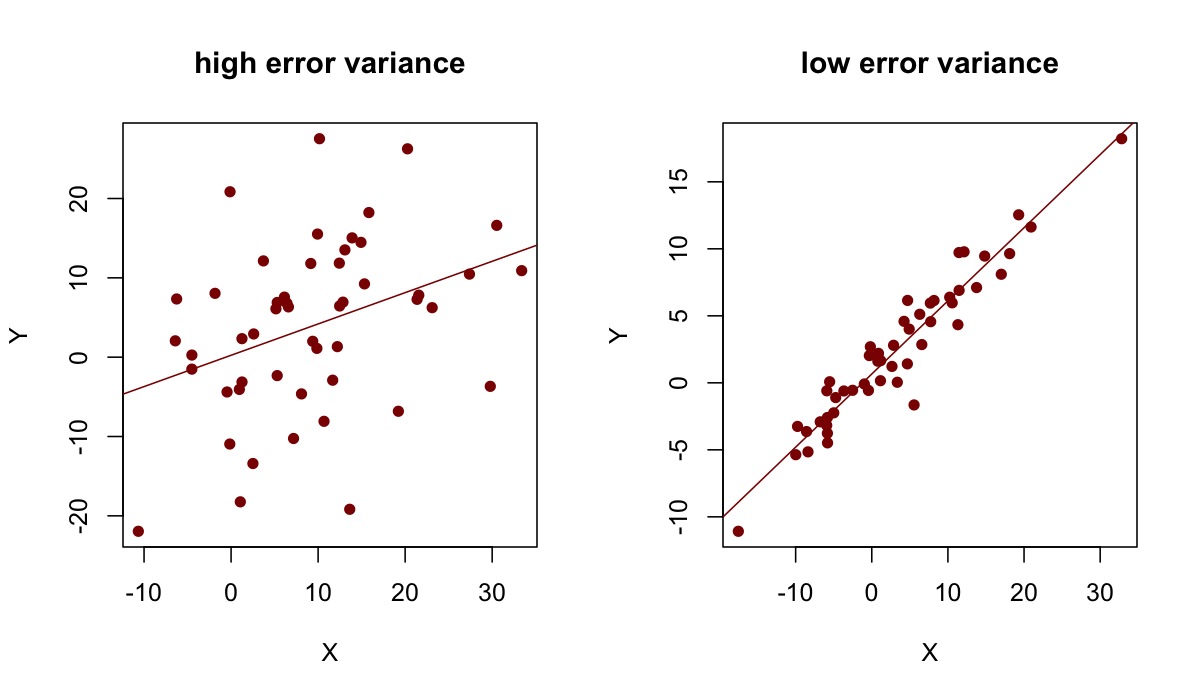
\includegraphics[width=0.8\linewidth]{low_v_high_1.png}
		\label{fig:low_v_high_1}
	\end{figure}}
	\only<3>{
	\begin{figure}[htpb]
		\centering
		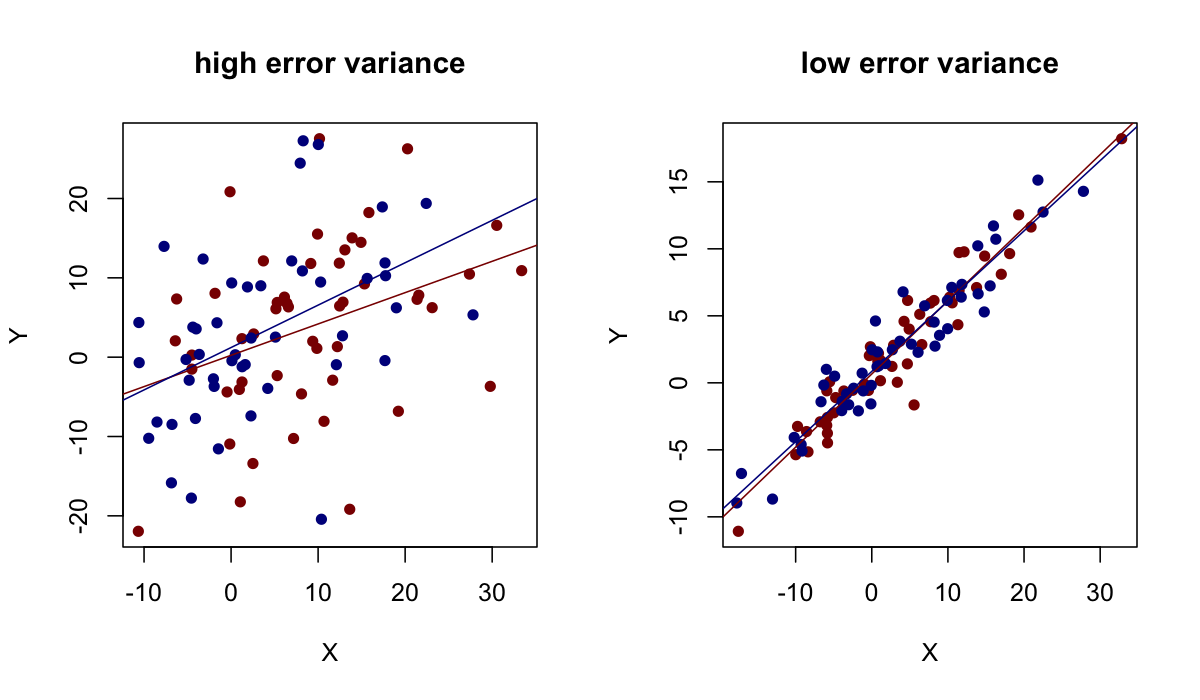
\includegraphics[width=0.8\linewidth]{low_v_high_2.png}
		\label{fig:low_v_high_2}
	\end{figure}}
	\only<4>{

	\ucla{Intuition:} If points are more tightly distributed around the regression line it is easier to tell what the regression line is.}
\end{frame}

\begin{frame}{Linear Regression: Asymptotic Variances} 
	\label{frame:variance2}
	For large \(n\) we have that
	\[
		\Var(\ucla{\hat\beta_1}) = \frac{\sigma_\eps^2}{n\cdot\sigma_X^2},\hbox{ }\Var(\ucla{\hat\beta_0}) = \sigma_\eps^2\frac{\E[X^2]}{n\cdot \sigma_X^2},\andbox \Cov(\ucla{\hat\beta_1},\ucla{\hat\beta_0}) = - \sigma_\eps^2 \frac{\E[X]}{n\cdot\sigma_X^2}  
	.\]
	These variances tend to zero as \(n\to \infty\); as we collect more data we are closer to the true values  \(\ucla{\beta_0}\) and \(\ucla{\beta_1}\).
	\only<2>{
	\begin{figure}[htpb]
		\centering
		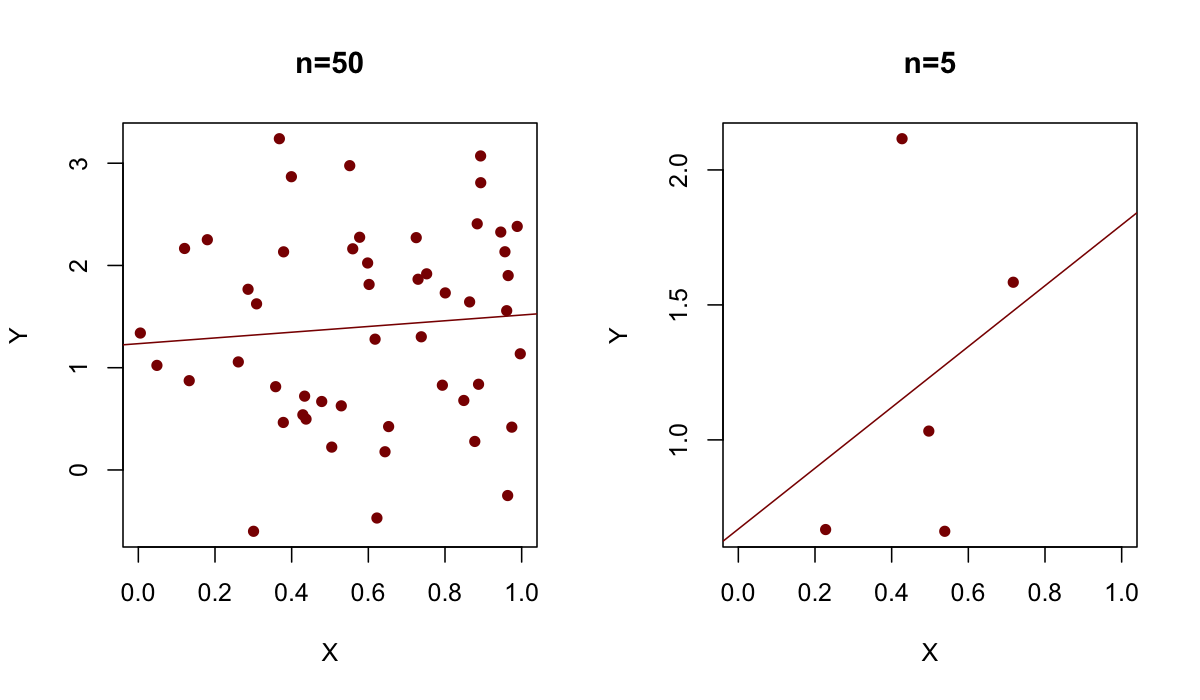
\includegraphics[width=0.8\linewidth]{low_v_high_n_1.png}
		\label{fig:low_v_high_1}
	\end{figure}}
	\only<3>{
	\begin{figure}[htpb]
		\centering
		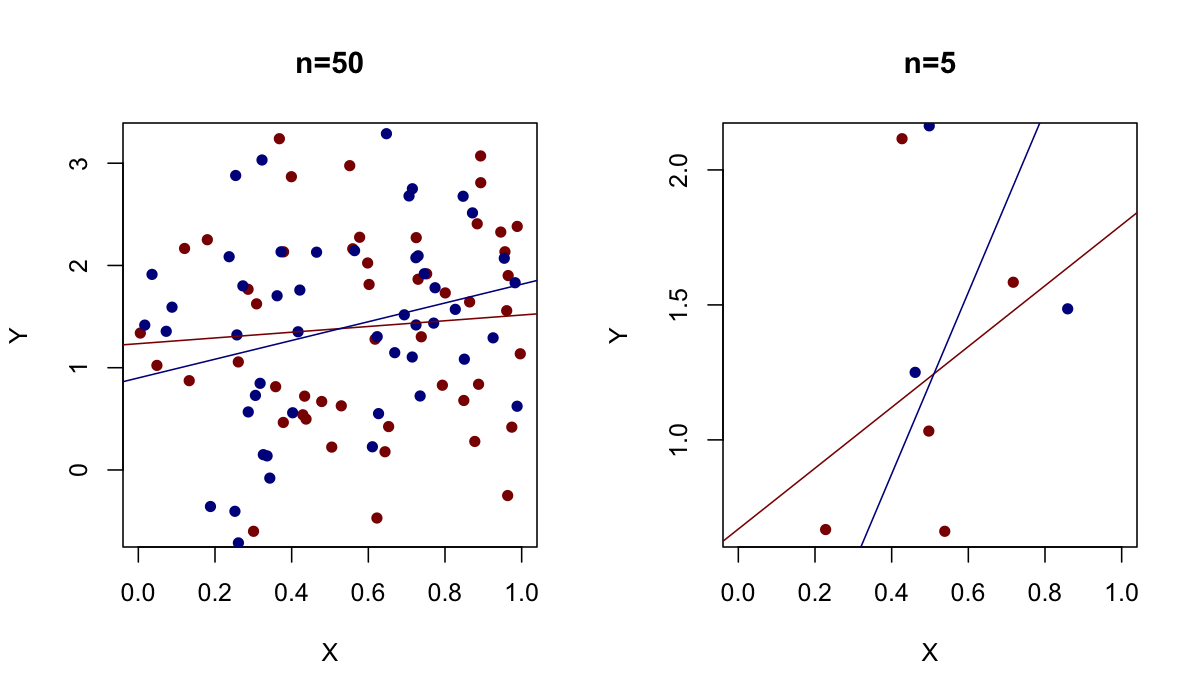
\includegraphics[width=0.8\linewidth]{low_v_high_n_2.png}
		\label{fig:low_v_high_2}
	\end{figure}}	
\end{frame}

\begin{frame}{Linear Regression: Asymptotic Variances} 
	\label{frame:variance3}
	For large \(n\) we have that
	\[
		\Var(\ucla{\hat\beta_1}) = \frac{\sigma_\eps^2}{n\cdot\sigma_X^2},\hbox{ }\Var(\ucla{\hat\beta_0}) = \sigma_\eps^2\frac{\E[X^2]}{n\cdot \sigma_X^2},\andbox \Cov(\ucla{\hat\beta_1},\ucla{\hat\beta_0}) = - \sigma_\eps^2 \frac{\E[X]}{n\cdot\sigma_X^2}  
	.\]
	These variances decrase as \(\sigma_X^2\) increases; as the spread of \(X\) increases we can make out the line more clearly.
	\only<2>{
	\begin{figure}[htpb]
		\centering
		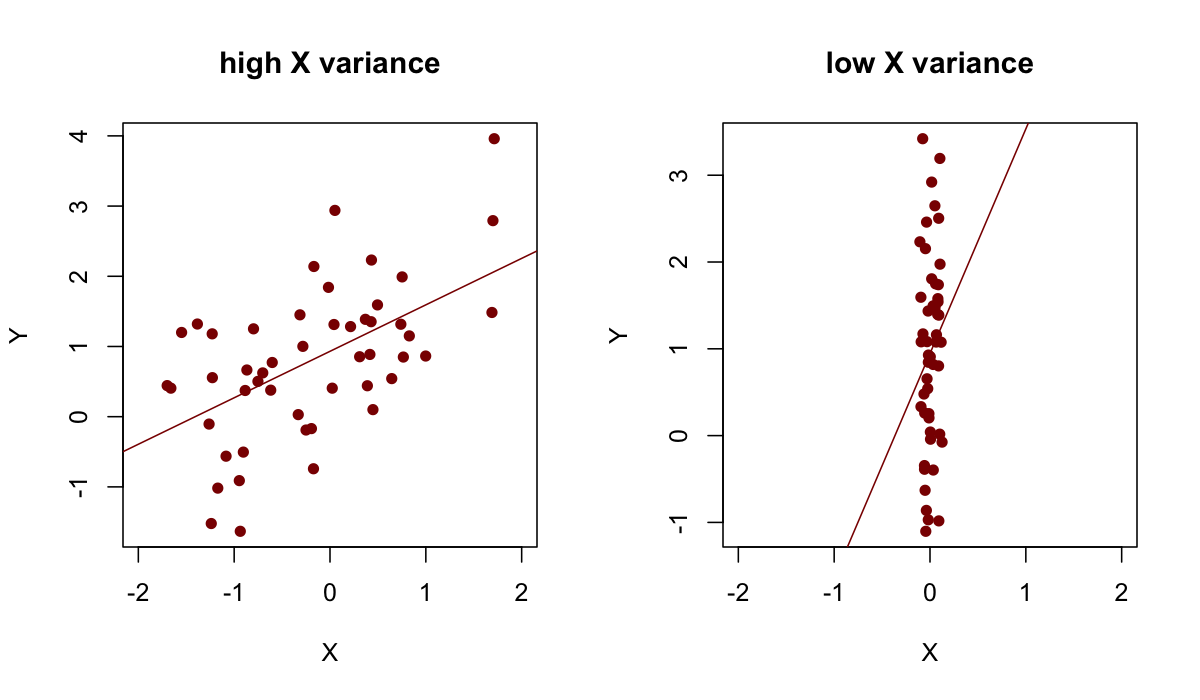
\includegraphics[width=0.8\linewidth]{low_v_high_x_1.png}
		\label{fig:low_v_high_1}
	\end{figure}}
	\only<3>{
	\begin{figure}[htpb]
		\centering
		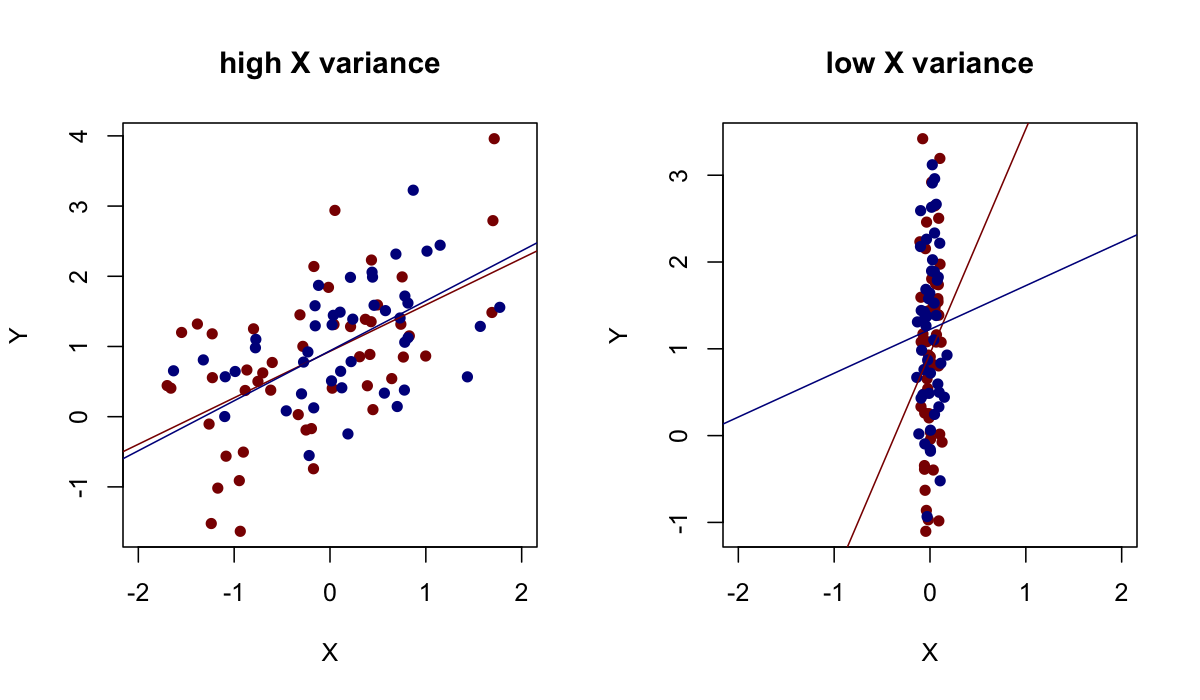
\includegraphics[width=0.8\linewidth]{low_v_high_x_2.png}
		\label{fig:low_v_high_2}
	\end{figure}}	
\end{frame}

\begin{frame}{Linear Regression: Questions}
	\centering
	\red{\Large Questions?}
\end{frame} 
\begin{frame}{Linear Regression: Variance Estimation} 
	\label{frame:variance-estimation}
	\ucla{Positive Result:} Under homoskedasticity, for \(n\) large, we have (approximately)
	\[
		\frac{\ucla{\hat\beta_1}-\ucla{\beta_1}}{\sigma_{\beta_1}/\sqrt{n}}  \sim N\left(0,1\right)
	.\] 
	where 
	\[
		\sigma_{\beta_1} = \frac{\sigma_\eps^2}{\sigma_X^2} 
	.\] 
	\onslide<2->
	\ucla{Problem:} What is \(\sigma_{\beta_1}\)? How can we estimate it?
	\begin{itemize}
		\item<3-> By \red{LLN} we know how to esimate \(\Var(X)\)
		 \[
			 \frac{1}{n}\sum_{i=1}^n (X_i - \bar X)^2 \approx \Var(X)
		.\] 
	\item<4-> But what about \(\Var(\eps) = \sigma_\eps^2\)?
	\end{itemize}
\end{frame}
\begin{frame}{Linear Regression: Variance Estimation} 
	\label{frame:variance-estimation2}
	To estimate \(\Var(\eps)\) we first construct estimated residuals \(\hat\eps_i\) via
	\[
	    \hat\eps_i = Y_i - \ucla{\hat\beta_0} - \ucla{\hat\beta_1}\cdot X_i
	.\]
	Because \(\ucla{\hat\beta_1} \to \ucla{\beta_1}\) and \( \ucla{\hat\beta_0} \to \ucla{\beta_0}\) we can say that \(\hat\eps_i \approx \eps_i = Y_i - \ucla{\beta_0} - \ucla{\beta_1}X_i\) (for \(n\) large). 
	
	\onslide<2-> 
	Also by the first order conditions for \(\ucla{\hat\beta_0}\) we have that
	\[
		- \frac{1}{n}\sum_{i=1}^n  (\underbrace{Y_i - \ucla{\hat\beta_0} - \ucla{\hat\beta_1}\cdot X_i}_{=\hat\eps_i}) = 0
	.\] 
	so that
	\[
		\frac{1}{n}\sum_{i=1}^n \hat\eps_i = \bar{\hat\eps}_i = 0
	.\] 
\end{frame}
\begin{frame}{Linear Regression: Variance Estimation} 
	\label{frame:variance-estimation3}
	Putting this together we can estimate \(\Var(\eps) = \sigma_\eps^2\) by calculating the sample variance of \(\hat\eps_i\):
	\begin{align*}
		\hat\sigma_\eps^2 &= \frac{1}{n}\sum_{i=1}^n \hat\eps_i^2 - \cancel{(\bar{\hat\eps}_i)^2} \\
		\onslide<2->{
		\intertext{By \(\ucla{\hat\beta_1}\to\ucla{\beta_1}\) and \( \ucla{\hat\beta_0}\to \ucla{\beta_0}\) as \(n\to\infty\);}
						  &\approx \frac{1}{n}\sum_{i=1}^n \eps_i^2}
		\onslide<3->{
		\intertext{By \red{Law of Large Numbers};}
						  &\approx \E[\eps^2] \\}
		\onslide<4->{
		\intertext{By \(\E[\eps] = 0\);}
						  &= \Var(\eps) = \sigma_\eps^2}
	\end{align*}
\end{frame}
\begin{frame}{Linear Regression: Variance Estimation} 
	\label{frame:variance-estimation4}
	Putting all of this together, we can estimate \(\sigma_{\beta_1}^2 = \frac{\sigma_X^2}{\sigma_X^2}\) via;
	\[
		\hat\sigma_{\beta_1}^2  = \frac{\hat\sigma_\eps^2}{\frac{1}{n}\sum_{i=1}^n (X_i - \bar X)^2} \approx \sigma_{\beta_1}^2
	.\] 
	since for large \(n\)
	\begin{align*}
		\hat\sigma_\eps^2 = \frac{1}{n}\sum_{i=1}^n \hat\eps_i^2 &\approx \sigma_{\eps}^2 \\ 
		\frac{1}{n}\sum_{i=1}^n (X_i - \bar X)^2 &\approx \sigma_X^2
	.\end{align*} 
\end{frame}
\begin{frame}{Linear Regression: Variance Estimation} 
	\label{frame:variance-estimation5}
	Now, since we have that (approximately, for large \(n\)):
	\[
		\frac{\ucla{\hat\beta_1}-\ucla{\beta_1}}{\sigma_{\beta_1}/\sqrt{n}} \sim N(0,1) 
	.\] 
	And since, as we have established above, \(\hat\sigma_{\beta_1} \approx \sigma_{\beta_1}\), for large \(n\) we can say that (approximately)
	\[
		\frac{\ucla{\hat\beta_1}-\ucla{\beta_1}}{\hat\sigma_{\beta_1}/\sqrt{n}}\sim N(0,1) 
	.\] 
\end{frame}
\begin{frame}{Linear Regression: Variance Estimation} 
	\label{frame:variance-estimation6}
	The quantity \(\hat\sigma_{\beta_1}/\sqrt{n}\) is often referred to as the \red{standard error} of \(\ucla{\hat\beta_1}\). 

	\onslide<4->
	\vfill
	In general, if we have a parameter \(\theta\) that we estimate with \(\hat\theta\), the quantity \(\hat\sigma_{\theta}/\sqrt{n}\) will be referred to as the \red{standard error} of \(\hat\theta\) where
	 \[
		 \hat\sigma_{\theta} = \sqrt{\Var(\hat\theta)}
	.\] 

\end{frame}



\begin{frame}{Variance Estimation: Questions}
	\centering
	\red{\Large Questions?}
\end{frame} 

\begin{frame}{Linear Regression: Why Asymptotic Distribution?} 
	\label{frame:why-useful}
	\onslide<1->
	Let's return to our example and see why this characterization is useful. Recall that in our example we are interested in the regression parameters from regression \(Y = INC\) (income in thousands of dollars) against  \(X = EDU\) (years of education).
	
	\onslide<2->
	After collecting a sample size of 100, \(\{Y_i,X_i\}_{i=1}^{100}\) we find that:
	\begin{align*}
		\ucla{\hat\beta_1} &= 0.5 \\
		\frac{1}{n}\sum_{i=1}^n \eps_i^2 &= 25\\
		\frac{1}{n}\sum_{i=1}^n (X_i - \bar X)^2 &= 16
	\end{align*}
	
\end{frame}
\begin{frame}{Linear Regression: Why Asymptotic Distribution?} 
	Our friend His Majesty Prince Harry claims there is no relationship between education and income, \( \ucla{\beta_1} = 0\). We claim that observing the magnitute of \(|\ucla{\hat\beta_1}|=0.5\) is evidence against this claim. Who is right?
	\begin{itemize}
		\item<2-> If \( \ucla{\beta_1}=0\) we would expect \(\ucla{\hat\beta_1}\) to be close to zero.
		\item<3-> But there is still some randomness in \(\ucla{\hat\beta_1}\), maybe we got \( \ucla{\hat\beta_1}= 0.5\) by chance.
	\end{itemize}
	\onslide<4->
	\vfill
	Want to use the (asymptotic) distribution of \(\ucla{\hat\beta_1}\) to answer this question. 
	\begin{itemize}
		\item<5-> First need to estimate \(\sigma_{\beta_1}\).
	\end{itemize}
\end{frame}
\begin{frame}{Linear Regression: Why Asymptotic Distribution?} 
	\label{frame:useful2}
	Using \(\hat\sigma_{\eps}^2 = \frac{1}{n}\sum_{i=1}^n \eps_i^2 = 25\), and \(\frac{1}{n}\sum_{i=1}^n (X_i - \bar X)^2 = 16)\) we calculate
	\begin{align*}
		\hat\sigma_{\beta_1}^2 
		&= \frac{\hat\sigma_\eps^2}{\frac{1}{n}\sum_{i=1}^n (X_i - \bar X)^2} \\
		&= \frac{25}{16} 
	\end{align*}
	\onslide<2->
	Using this, we find that \(\hat\sigma_{\beta_1} = \sqrt{\hat\sigma_{\beta_1}^2} = \frac{5}{4} \).
\end{frame}
\begin{frame}{Linear Regression: Why Asymptotic Distribution?} 
	\label{frame:useful3}
	Now recall that for \(n\) large we have that (approximately)
	\[
		\frac{\ucla{\hat\beta_1}-\ucla{\beta_1}}{\hat\sigma_{\beta_1}/\sqrt{n}}\sim N(0,1) 
	.\] 
	\onslide<2->
	If the true value of  \( \ucla{\beta_1} = 0\) this means that 
	\[
		\frac{\ucla{\hat\beta_1}}{5/40} = \frac{\ucla{\hat\beta_1}}{0.125}  \sim N(0,1)
	.\] 	
\end{frame}
\begin{frame}{Linear Regression: Why Asymptotic Distribution?} 
	\label{frame:useful4}
	Given that if \( \ucla{\beta_0}=0\),  \(\ucla{\hat\beta_1}/0.125 \sim N(0,1)\), what is the probability of us observing \( |\ucla{\hat\beta_1}| \geq  0.5\)?
	\begin{align*}
		\onslide<2->{\Pr\left(|\ucla{\hat\beta_1}|\geq 0.5 \right) &= \Pr\left(|\ucla{\hat\beta_1}/0.125| \geq 0.5/0.125\right)\\}
		\onslide<3->{&= \Pr(|Z| \geq 4)\intertext{where \(Z\sim N(0,1)\)}}
		\onslide<4->{&= \Pr(Z \geq 4) + \Pr(Z \leq 4) \\ &= 2\Pr(Z \geq 4)\intertext{By symmetry of the normal distribution}}
		\onslide<5->{&\approx 0.00006 }
	\end{align*}
\end{frame}
\begin{frame}{Linear Regression: Why Asymptotic Distribution?} 
	\label{frame:useful5}
	Using the asymptotic distribution result
	\[
		\frac{\ucla{\hat\beta_1}-\ucla{\beta_1}}{\hat\sigma_{\beta_1}/\sqrt{n}} \sim N(0,1) 
	,\] 
	we have found that if \( \ucla{\beta_1} = 0\), then \(\Pr(|\ucla{\hat\beta_1}| \geq 0.5) \approx 0.0006\).
	\vfill\onslide<2->
	So, given that we observed \(\ucla{\hat\beta_1}=0.5\), it seems very unlikely that \( \ucla{\beta_1}=0\). We can conclude against Prince Harry's claim.
\end{frame}
\begin{frame}{Asymptotic Distribution: Questions}
	\centering
	\red{\Large Questions?}
\end{frame} 

\section{Hypothesis Testing and Confidence Intervals}

\begin{frame}{Linear Regression: Hypothesis Testing} 
	\label{frame:hyp1}
	The last exercise where we tested whether Prince Harry's claim made sense was an example of a \red{hypothesis test}.
	
	In this section we will formally discuss hypothesis testing. 
\end{frame}
\begin{frame}{Linear Regression: Hypothesis Testing} 
	\label{frame:hyp2}
	Often in linear regression analysis, we are interested in 
\end{frame}

\end{document}


